% Drawing 154/02-7 -- folder 154, batch 02, archive page 29 (PDF page 30).
% Transcription: page de dessins, sans texte : cinq disques au bord vert, chacun traversé d'un arrangement de pseudo-droites orange, accolés les uns aux autres en chaîne autour d'un point où les bords se rejoignent ; sur l'un des bords, un arc vert foncé fléché porte les lettres $p$, $q$ et un troisième signe \uncertain{peu net} ; hachures et gribouillis au crayon sur deux disques --- recollement des disques $\Delta(D)$ décrit pages 25 et 27
% Kind: chain of five disks with pseudoline arrangements, glued around a point. Method 2 (schematic redraw from the facsimile). Status: partial.
% Notes: Five disks with green rims, each crossed by an orange arrangement, glued to one another in a chain around a point where the rims meet; on the rims, dark green arrowed arcs, one carrying the letters p, q and a third sign (read « p », « q » only); pencil hatching and scribble on two disks. The disks and the arrowed arcs are placed as on the page; the orange arrangements are schematic (a few strands per disk). Over a printed job listing (not reproduced). Read from the page view.
% Coordinates: 1 unit = 1 mm = 1/100 of the crop width (bbox in page fractions: [0.547, 0.143, 0.918, 0.403]).
% Redrawn by Claude (claude-opus-5-5), issue #73, 2026-11-07; not checked by a human; not compiled (no TeX in the session).
% Rights: reproduces part of the work -- behind RENDER_TRANSCRIPTS, never published by itself.
\documentclass[tikz,border=3pt]{standalone}
\usepackage{amsmath,amssymb}
\usetikzlibrary{patterns,arrows.meta}
\tikzset{Or/.style={orange!90!black}, Ye/.style={yellow!80!orange}, Lg/.style={green!60!black!70}, Dg/.style={green!45!black}, Br/.style={brown!80!black}, Rd/.style={red!85!black}, Bl/.style={blue!70!black}, Gy/.style={black!40}, pencil/.style={black!45}, struck/.style={black!35}, mark/.style={circle,draw,inner sep=1.3pt}, pt/.style={circle,fill,inner sep=0.9pt}, opt/.style={circle,draw,fill=white,inner sep=1.1pt}}
\begin{document}
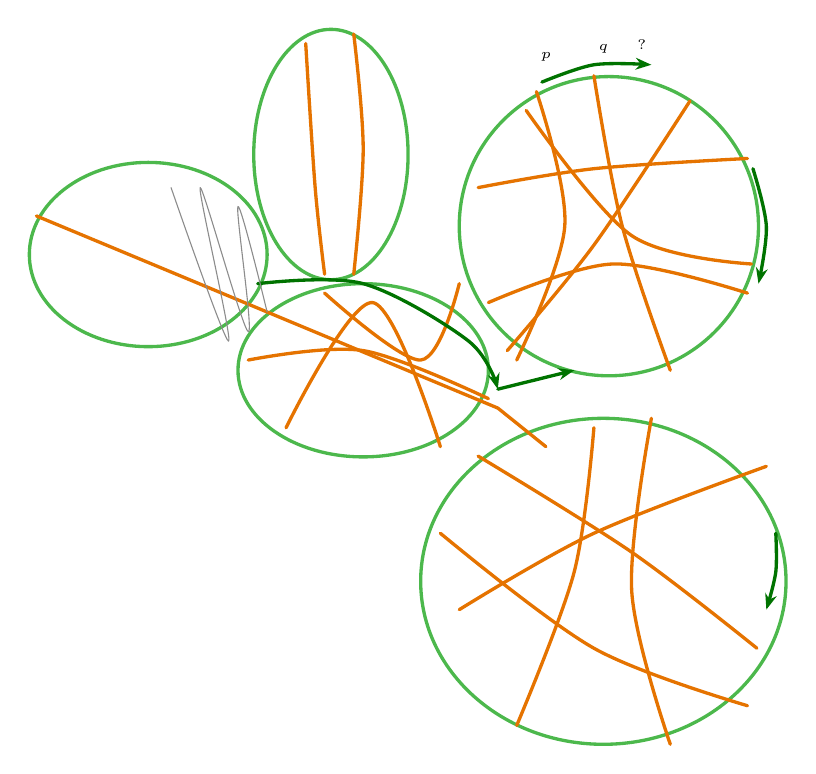
\begin{tikzpicture}[x=1mm,y=1mm,line cap=round,line join=round,font=\scriptsize]
\draw[Lg,very thick] (16.6,-32.9) ellipse[x radius=15.1, y radius=11.7];
\draw[Lg,very thick] (39.8,-20.2) ellipse[x radius=9.8, y radius=15.9];
\draw[Lg,very thick] (43.9,-47.6) ellipse[x radius=15.9, y radius=11];
\draw[Lg,very thick] (75.1,-29.3) circle[radius=19];
\draw[Lg,very thick] (74.4,-74.4) ellipse[x radius=23.2, y radius=20.7];
\draw[Or,very thick] (2.4,-28) -- (61,-52.4);
\draw[Or,very thick] plot[smooth, tension=0.55] coordinates {(36.6,-6.1) (37.8,-24.4) (39,-35.4)};
\draw[Or,very thick] plot[smooth, tension=0.55] coordinates {(42.7,-4.9) (43.9,-19.5) (42.7,-35.4)};
\draw[Or,very thick] plot[smooth, tension=0.55] coordinates {(29.3,-46.3) (43.9,-45.1) (59.8,-51.2)};
\draw[Or,very thick] plot[smooth, tension=0.55] coordinates {(34.1,-54.9) (45.1,-39) (53.7,-57.3)};
\draw[Or,very thick] plot[smooth, tension=0.55] coordinates {(39,-37.8) (51.2,-46.3) (56.1,-36.6)};
\draw[Or,very thick] plot[smooth, tension=0.55] coordinates {(58.5,-24.4) (73.2,-22) (92.7,-20.7)};
\draw[Or,very thick] plot[smooth, tension=0.55] coordinates {(59.8,-39) (75.6,-34.1) (92.7,-37.8)};
\draw[Or,very thick] plot[smooth, tension=0.55] coordinates {(65.9,-12.2) (69.5,-29.3) (63.4,-46.3)};
\draw[Or,very thick] plot[smooth, tension=0.55] coordinates {(73.2,-10.2) (76.8,-29.3) (82.9,-47.6)};
\draw[Or,very thick] plot[smooth, tension=0.55] coordinates {(85.4,-13.4) (73.2,-31.7) (62.2,-45.1)};
\draw[Or,very thick] plot[smooth, tension=0.55] coordinates {(64.6,-14.6) (78,-30.5) (93.2,-34.1)};
\draw[Or,very thick] plot[smooth, tension=0.55] coordinates {(58.5,-58.5) (78,-70.7) (93.9,-82.9)};
\draw[Or,very thick] plot[smooth, tension=0.55] coordinates {(56.1,-78) (73.2,-68.3) (95.1,-59.8)};
\draw[Or,very thick] plot[smooth, tension=0.55] coordinates {(63.4,-92.7) (70.7,-73.2) (73.2,-54.9)};
\draw[Or,very thick] plot[smooth, tension=0.55] coordinates {(80.5,-53.7) (78,-75.6) (82.9,-95.1)};
\draw[Or,very thick] plot[smooth, tension=0.55] coordinates {(53.7,-68.3) (73.2,-82.9) (92.7,-90.2)};
\draw[Or,very thick] (61,-52.4) -- (67.1,-57.3);
\draw[Dg,very thick,-{Stealth[length=2mm]}] plot[smooth, tension=0.55] coordinates {(30.5,-36.6) (43.9,-36.6) (57.3,-43.9) (61,-50)};
\draw[Dg,very thick,-{Stealth[length=2mm]}] plot[smooth, tension=0.55] coordinates {(66.6,-11) (73.2,-8.8) (80.5,-8.8)};
\draw[Dg,very thick,-{Stealth[length=2mm]}] plot[smooth, tension=0.55] coordinates {(93.4,-22) (95.1,-29.3) (94.1,-36.6)};
\draw[Dg,very thick,-{Stealth[length=2mm]}] plot[smooth, tension=0.55] coordinates {(96.3,-68.3) (96.3,-73.2) (95.1,-78)};
\draw[Dg,very thick,-{Stealth[length=2mm]}] (61,-50) -- (70.7,-47.6);
\node[inner sep=1pt] at (67.1,-7.8) {\tiny $p$};
\node[inner sep=1pt] at (74.4,-6.8) {\tiny $q$};
\node[inner sep=1pt] at (79.3,-6.3) {\tiny $?$};
\draw[pencil] plot[smooth, tension=0.55] coordinates {(19.5,-24.4) (26.8,-43.9) (23.2,-24.4) (29.3,-42.7) (28,-26.8) (31.7,-40.2)};
\end{tikzpicture}
\end{document}
